% ****** Start of file apssamp.tex ******
%
%   This file is part of the APS files in the REVTeX 4.1 distribution.
%   Version 4.1r of REVTeX, August 2010
%
%   Copyright (c) 2009, 2010 The American Physical Society.
%
%   See the REVTeX 4 README file for restrictions and more information.
%
% TeX'ing this file requires that you have AMS-LaTeX 2.0 installed
% as well as the rest of the prerequisites for REVTeX 4.1
%
% See the REVTeX 4 README file
% It also requires running BibTeX. The commands are as follows:
%
%  1)  latex apssamp.tex
%  2)  bibtex apssamp
%  3)  latex apssamp.tex
%  4)  latex apssamp.tex
%
\documentclass[%
 reprint,
%superscriptaddress,
%groupedaddress,
%unsortedaddress,
%runinaddress,
%frontmatterverbose, 
%preprint,
%showpacs,preprintnumbers,
%nofootinbib,
%nobibnotes,
%bibnotes,
 amsmath,amssymb,
 aps,
%pra,
%prb,
%rmp,
%prstab,
%prstper,
%floatfix,
]{revtex4-1}
\usepackage{xcolor}
\usepackage{graphicx}% Include figure files
\usepackage{dcolumn}% Align table columns on decimal point
\usepackage{bm}% bold math
%\usepackage{hyperref}% add hypertext capabilities
%\usepackage[mathlines]{lineno}% Enable numbering of text and display math
%\linenumbers\relax % Commence numbering lines

%\usepackage[showframe,%Uncomment any one of the following lines to test 
%%scale=0.7, marginratio={1:1, 2:3}, ignoreall,% default settings
%%text={7in,10in},centering,
%%margin=1.5in,
%%total={6.5in,8.75in}, top=1.2in, left=0.9in, includefoot,
%%height=10in,a5paper,hmargin={3cm,0.8in},
%]{geometry}
\usepackage[spanish]{babel}
\usepackage[utf8]{inputenc}
\usepackage{float}
\providecommand{\e}[1]{\ensuremath{\times 10^{#1}}} %Notacion cientifica
\usepackage{textcomp}
\usepackage{longtable}
%\usepackage{multicol}
\usepackage{lipsum, babel}
\newcommand{\specialcell}[2][c]{%
  \begin{tabular}[#1]{@{}c@{}}#2\end{tabular}}
 \usepackage{graphicx}

 
\begin{document}
\title{Estudio del comportamiento termodinámico de la membrana de \textit{Staphylococcus aureus} por la técnica FTIR}% Force line breaks with \\
%\thanks{\url{https://github.com/dforero0896/Laboratorio_Intermedio/tree/master/Radiactividad}}%

\author{John Erick Cabrera Ramirez}
 \affiliation{Universidad de Los Andes}%Lines break automatically or can be forced with \\


\date{\today}% It is always \today, today,
             %  but any date may be explicitly specified

\begin{abstract}
\begin{center}
  \textit{Resumen}  
\end{center}

Se estudian cambios en la transición de fase sólido ordenado a líquido desordenado en sistemas de membranas modelo DPPC con el fin de estudiar posteriormente la membrana de  \textit{Staphylococcus aureus} en presencia o ausencia del carotenoide estafiloxantina. La transición de fase se estudia usando la técnica de espectrofotometría infrarroja por transformada de Fourier (FTIR) y se determina haciendo seguimiento del número de onda de la banda de absorción CH$_{2}$ de los ácidos grasos en función de la temperatura. Para la banda de absorción de DPPC no se encuentra un punto de inflexión en el centro de la temperatura de transición. Por otro lado, como se medirá el espectro para membranas de \textit{Staphylococcus aureus} se buscan los puntos óptimos de trabajo en las curvas de crecimiento, para la cepa nativa se encontró que es alrededor de 12 horas, sin embargo para las cepas que producen carotenoides en exceso y las que no lo producen los resultados no son concluyentes. Deben realizarse de nuevo sus curvas de crecimiento. Adicionalmente, se medirá el nivel de cooperatividad de la transición de fase mediante la  determinación del ancho de banda en la curva de la primera derivada.

\end{abstract}

\pacs{Valid PACS appear here}% PACS, the Physics and Astronomy
                             % Classification Scheme.
%\keywords{Suggested keywords}%Use showkeys class option if keyword
                              %display desired
\maketitle

%\tableofcontents


%TC:endignore
\section{\label{sec:intro}Introducción y Estado del Arte}
%\subsection{\textit{S. Aureus} y su Membrana}
\textit{Staphylococcus aureus} es una bacteria patógena (que causa enfermedades infecciosas) tipo Gram-positiva, ver figura \ref{fig:sta},  la cual se encuentra en la microbiota humana sin producir enfermedades en condiciones normales, pero que en condiciones desfavorables tales como heridas y cicatrices operatorias puede causar o estar relacionada con enfermedades de diferente gravedad en el sistema respiratorio, en los tejidos blandos y en el torrente sanguíneo \cite{1HarpavatS.NissimS.LipppincottsMicrocards:MicrobiologyFlashCards2012.}.\\
\begin{figure}[h]
  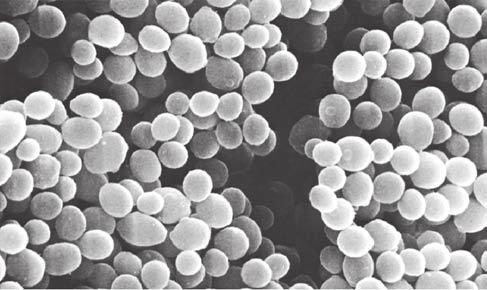
\includegraphics[width=\linewidth]{s_aureus.jpg}
  \caption{Fotografía  de \textit{Staphylococcus aureus}. Tomado de \cite{1HarpavatS.NissimS.LipppincottsMicrocards:MicrobiologyFlashCards2012.}}
  \label{fig:sta}
\end{figure}

Desde el descubrimiento de \textit{S. aureus} como causante de una infección a una herida en 1881 \cite{Orent2006AMagazine}, se ha investigado su presencia en otras infecciones y se han utilizado antibióticos como la penicilina y la meticilina para controlar estas infecciones \cite{1HarpavatS.NissimS.LipppincottsMicrocards:MicrobiologyFlashCards2012.}. Sin embargo \textit{S. aureus} ha desarrollado resistencia a estos antibióticos,  surgiendo la necesidad de buscar nuevos antibióticos, entre los cuales se encuentran los péptidos antimicrobianos.\\
Los péptidos antimicrobianos interactúan con la membrana de la bacteria produciendo orificios que causan pérdida de contenido y muerte celular. La resistencia a los poros. Para entender como puede generar resistencia a estos antibióticos es importante estudiar la rigidez mecánica y la elasticidad de la membrana. Adicionalmente, se sabe que la composición de la bicapa lipídica de la membrana de \textit{S. aureus} cambia de manera adaptativa al medio ambiente, volviéndose más resistente como respuesta a estrés externo.\\
\textit{S. aureus} al ser una bacteria Gram positiva tiene expuesto al exterior un compuesto llamado peptidoglicando. La membrana celular que recubre la bacteria es una bicapa fosfolipídica que contiene dos capas de glicerofosfolípidos. Los glicerofosfolípidos son moléculas anfipáticas, las cuales tienen una parte hidrofóbica y otra parte hidrofílica \cite{Nelson2011}, al ser anfipáticas la parte interna de la bicapa es hidrofóbica mientras que la parte externa de la membrana es hidrofílica.La interacción lateral entre estas moléculas se da través de fuerzas no covalentes lo que le confiere propiedades de cristal líquido caracterizado por la capacidad de presentar transiciones de fase sólido-líquido. \\
La membrana de \textit{S. aureus} está compuesta principalmente por  fosfatidiletalonamina, cardiolipina, fosfatidilglicerol y estafiloxantina \cite{Ocampo2010TheAureus}, siendo la estafiloxantina un carotenoide que le da el color dorado (aúreo) característico de \textit{S. aureus}. Además, dependiendo de la composición específica de la membrana celular dicha membrana va a ser más o menos rígida lo cual implica corrimientos en la temperatura de transición y cambios en la cooperatividad de la transición de fase. La estructura molecular de los fosfolípidos presentes en la membrana hace que esta sea más fluida cuando la estructura presenta moléculas con múltiples insaturaciones que inducen un incremento en espaciamiento, reduciendo la interacción entre ellas. La membrana puede pasar de un estado sólido-ordenado (so) a un estado líquido-desordenado (ld) con un incremento de temperatura. En el caso de \textit{S. aureus} se ha descubierto que su membrana cambia el estado de rigidez de su membrana modulando la cantidad de estafiloxantinas presentes y la cantidad de cardiolipinas. \\
En cuanto a la fluidez de la membrana de acuerdo a la temperatura, si se estudia una membrana compuesta únicamente por glicerofosfolípidos, tal como se muestra en \cite{Heimburg}, esta presenta diferentes estados de acuerdo a su temperatura:  laminar líquido cristalino, gel laminar, laminar ondulada, entre otras.

Debido a la importancia de la rigidez de la membrana lipídica en los procesos de defensa de la célula e incluso para la búsqueda de nuevos antibióticos, el objetivo principal es estudiar la transición de fase sólido-ordenado/líquido-desordenado de la membrana de S.aureus en presencia y ausencia de estafiloxantina con base en gráficas de posición de la banda CH$_{2}$ asimétrico en función de la temperatura.\\
Para enteder la transición de fase de una membrana en un sistema vivo, primero se estudia la transición fase en un sistema modelo compuesto por un solo tipo de lípidos.
\subsection{Transiciones de Fase en Lípidos}
En solución con agua, los lípidos tienden a formar agregados debido a  su carácter anfipático. Para concentraciones mucho mayores a cierta concentración crítica \cite{Heimburg}, los lípidos tienden a formar bicapas. Las fases de estas bicapas se conocen como fases laminares y según su incremento en la temperatura se clasifican en:
\begin{itemize}
    \item \textit{Fase} $L_{c}$: Los lípidos forman bicapas que presentan un orden en las tres dimensiones, es decir, las cabezas polares del lípido presentan un patrón en forma de red mientras que las cadenas apolares están ordenadas en configuración  trans.
    \item  \textit{Fase} $L_{\beta'}$: Esta es conocida como la fase gel. En esta los lípidos se encuentran mayoriatariamente ordenados pero no todas cadenas hidrocarbonadas son trans. Se llama $\beta'$ porque algunos lípidos presentan una inclinación respecto al plano de la normal, \cite{Heimburg}.
    \item  \textit{Fase} $P_{\beta '}$: Esta fase es una mezcla entre las fases de gel $L_{\beta '}$ y fluida $L_{\alpha}$. Se denomina así porque la membrana presenta ondulaciones periódicas.
      \item  \textit{Fase} $L_{\alpha}$: Esta es la fase líquida o fluida de la membrana donde no hay un orden lateral de los grupos polares ni en las cadenas hidrocarbonadas.
\end{itemize}
Cuando ocurre una transición de fase de primer orden, la presión y la temperatura son aproximadamente constantes. El calor específico a presión constante se calcula mediante la relación:
\begin{equation}
    c_{p}=\left(\frac{\partial H}{\partial T}\right)_{P}
\end{equation}\label{eq:1}
Donde $H$ es la entalpía del sistema, en este caso de la membrana bacteriana. Cuando ocurre la transición de fase, hay un salto de la entalpía. Cuando hay un salto en la entalpía, el calor específico $c_{p}$ presenta un pico, como una función tipo aguja.\\
Para liposomas con un solo lípido se encuentran mediante métodos de calorimetría las curvas de calor específico mostradas en la figura \ref{fig:esp3}. Los tres compuestos son dimiristoil fosfatidilcolina ( por sus siglas en inglés DMPC), dipalmitoilfosfatidilcolina ( por sus siglas en inglés DPPC) y diasteroilfosfatidilcolina ( por sus siglas en inglés DSPC).
\begin{figure}[h]
  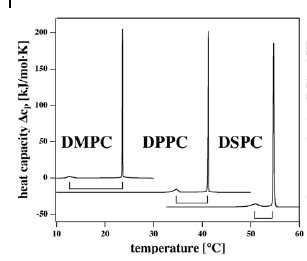
\includegraphics[width=\linewidth]{cp.png}
  \caption{ Calor específico en función de la temperatura para tres lípidos diferentes. Los picos representan la transición de fase cada uno.Tomado de \cite{Heimburg}}.
  \label{fig:esp3}
\end{figure}
 Como la composición de la bicapa fosfolipídica de \textit{S. aureus} no contiene únicamente el mismo tipo de fosfolípidos, sino principalmente los que se han mencionado previamente, entonces no se espera obtener una transición de fase con un salto perfecto, sino que tenga un ancho de banda tal como se muestra en la figura \ref{fig:ent2}, para más detalles ver \cite{Ocampo2010TheAureus}.\\
\begin{figure}[h]
  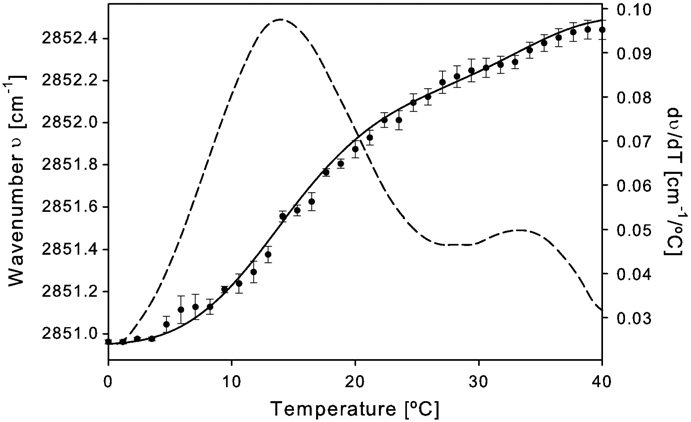
\includegraphics[scale=0.3]{transicion.png}
  \caption{ Número de onda de la banda de CH$_{2}$ en función de la temperatura y su derivada para la membrana de \textit{S. aureus}. Imagen tomada de \cite{Ocampo2010TheAureus}.}
  \label{fig:ent2}
\end{figure}
En la figura \ref{fig:ent2} cabe destacar que el número de onda es directamente proporcional a la energía de vibración de las moléculas debido a la relación $E=h\nu$ con $\nu$ la frecuencia de vibración.\\
La gráfica \ref{fig:ent2} se obtuvo mediante la técnica de espectroscopía de FITR variando la temperatura de la muestra.
\subsection{Espectrofotómetro de transformada de Fourier en el infrarrojo (FTIR)}
Es un instrumento basado en el interferómetro de Michelson cuyo objetivo es medir el espectro de absorción y/o de emisión de una muestra en el infrarrojo. En el espectrofotómetro dos haces policromáticos  toman diferentes caminos ópticos. La diferencia de fases es una medida de la intensidad de luz que sale de la muestra. La idea de producir la diferencia de fases es que uno de los haces pase por la muestra. Se llama (IR) de rayos infrarrojos porque el barrido de longitudes de onda que hace el espectrofotómetro es sobre el infrarrojo.
En la figura \ref{fig:FTIR} se muestra el esquema de un FTIR la cual se discute a continuación.
\begin{figure}[h]
  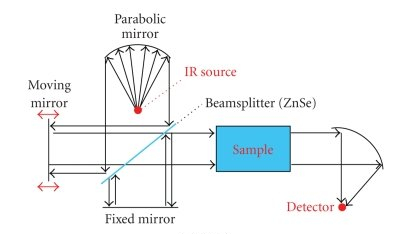
\includegraphics[width=\linewidth]{FTIR.jpg}
  \caption{Esquema de un FTIR. Figura tomada de \cite{Downes2010}.}
  \label{fig:FTIR}
\end{figure}
\subsection{Curvas de Crecimiento}
Con el fin de medir las transiciones de fase, se desea buscar el punto óptimo en el cual la población de células vivas sea mayor a la de células muertas y además nos encontremos cerca del equilibrio poblacional.\\
Desde el siglo XIX es bien conocido que una población bacteriana sigue cuatro fases \cite{Unknowna} denominadas \textit{fase de adaptación} (lag),  \textit{fase exponencial},  \textit{fase de estacionaria} y muerte celular o fase de decrecimiento logarítmico. Las primeras tres fases se han modelado mediante la ecuación logística \cite{Zill2009} que tiene en cuenta el crecimiento exponencial y la competencia. La solución de la ecuación logística en este caso es una curva sigmoidal de la forma:
\begin{equation}
    P(t)=\frac{aP_{0}}{bP_{0}+(a-bP_{0})e^{-at}},
\end{equation}\label{eq:2}
donde $P(\infty)=a/b$
Una curva de crecimiento tiene la forma mostrada en la figura .
\begin{figure}[h]
  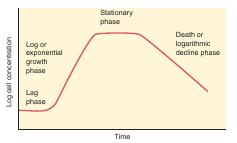
\includegraphics[width=\linewidth]{curva.png}
  \caption{Fases de una curva de crecimiento en escala log. Las primeras tres fases se modelan como una sigmoidal. Figura tomada de \cite{Unknowna}.}
  \label{fig:curv}
\end{figure}
\section{\label{sec:exp}Marco Experimental}
Para estudiar la transición de fase sólido-ordenado/líquido-desordenado de la membrana de S.aureus en presencia y ausencia de estafiloxantina se plantea obtener gráficas de posición de la banda CH$_{2}$ asimétrico en función de la temperatura.

\subsection{Curva de Crecimiento}
Se toman tres cepas de \textit{S. aureus}, la nativa llamada 144, una que mediante un plásmido produce un exceso de carotenoides (incluido estafiloxantina) llamada 147 y otra que es un mutante (knockout) del gen crtM de la ruta de síntesis, que no produce estafiloxantina llamada 145.A las tres cepas se les realiza una curva de crecimiento.  Esto se realiza con el fin de conocer cual es la fase estacionaria de la curva que va a ser el punto óptimo de trabajo. Para dicha tarea se recuperan las células que están a -80\textdegree C, es decir, se toma una colonia y se cultivan en cajas Petri que contienen LB-agar. Luego se toma una colonia de la caja Petri, se diluye en 10mL de LB líquido y se deja en overnight dentro del agitador ``Shaker'' a  37\textdegree C, ver figura \ref{fig:curv1}.\\
\begin{figure}
 \input{esquema1.pdf_tex}
  \caption{Algunos pasos para realizar una curva de crecimiento.}
  \label{fig:curv1}
\end{figure}
 Al tomar una gota de la dilución dejada en overnight, se puede conocer el número de células contenidas en la gota usando el nanodrop o un espectrofotómetro, el número de células será proporcional a la absorbancia.\\
 Para realizar la curva de crecimiento de la cepa 145 se utiliza la dilución de la cepa en 10mL de LB adicionándole el antibiótico cloranfenicol a 20\% V/V.\\
 Para la cepa 147 se agrega a la dilución con bacterias el antibiótico eritromicina a una concentración  de 2$\mu$g/mL.
 \subsection{Espectro FTIR}
Antes de trabajar con un sistema \textit{in vivo} se miden los espectros para liposomas hechos de  DMPC en función de la temperatura, esto en parte para verificar el funcionamiento del control de temperatura y en parte como comparación del sistema modelo al vivo. El control de temperatura tiene un encapsulado en cuyo interior hay una lámina de Cu que calienta la muestra y vidrios de Ge transparentes al infrarrojo. En el centro de las dos láminas de Ge se coloca la muestra.  La temperatura se variará por debajo de la temperatura ambiente (aproximadamente desde 8\textdegree C) y por encima de la temperatura ambiente ( abajo de 40\textdegree C aproximadamente) en pasos de a 5 \textdegree C cada minuto, ver \cite{Ocampo2010TheAureus}. Para tomar el espectro por cada temperatura se acopla el control de temperatura al FTIR, tal como se ilustra en la figura \ref{fig:mont2}.\\
\begin{figure}
 \input{esquema2.pdf_tex}
  \caption{Esquema del control de temperatura acoplado al FTIR usado para medir el espectro en función de la temperatura.}
  \label{fig:mont2}
\end{figure}
Una vez trabajado los liposomas de DPPC\footnote{Liposomas proporcionados por el grupo de biofísica}, se mide el espectro de las tres cepas 144, 145 y 147. Para esto, debe tenerse en cuenta la curva de crecimiento. Con la curva se establece el punto de crecimiento óptimo de las células a trabajar. Una vez escogido este punto, se coloca una muestra de \textit{S. aureus} en el interior del control de temperatura \footnote{Mediciones realizadas con la colaboración del grupo de química aromática de la universidad},  y se miden los espectros para cada temperatura tal como se describió antes.
Se busca en la curva del espectro de absorbancia el pico correspondiente a la vibración asimétrica de CH$_{2}$ el cual está alrededor de $2853 \mathrm{cm}^{-1}$ y se mide el valor del número de onda de este pico en función de la temperatura. La temperatura es el parámetro controlable mediante la interfaz que conecta al computador.
\section{Resultados Preliminares y An\'alisis}
Las curvas de crecimiento obtenidas para las cepas 144 y 145 son las mostradas en la gráfica \ref{fig:cur1}. Las densidades ópticas en función del tiempo para la 144 y la 145 (día 1) son la verde y la roja respectivamente; estas fueron tomadas hasta que se visualizara un cambio de concavidad en las curvas, lo cual ocurrió alrededor de las 12 horas. Los puntos más altos que están al inicio representan los valores de la densidad óptica del overnight. Se espera que las curvas alcancen este valor de la densidad óptica cuando lleguen a la fase estacionaria. La curva de la cepa 147 se intentó realizar pero no creció.\\
\begin{figure}[h]
 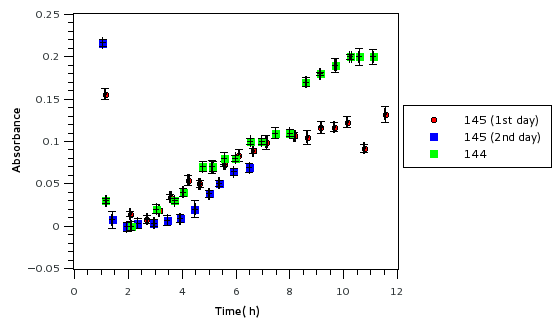
\includegraphics[width=\linewidth]{curvas/gratodas.png}
  \caption{Curvas de crecimiento para las cepas 144 y 145}
  \label{fig:cur1}
\end{figure}
 A pesar de que la cepa 145 se cultivó en cloranfenicol, se esperaba que esta tuviera un tiempo de adaptación (lag phase) más prolongado que el de la 144 ya que la cepa 145 no produce carotenoides. Con base en esto, se decide tomar nuevamente los datos de la curva 145, representada en la gráfica  \ref{fig:cur1} como 145 (día 2) en azul. Se observa que la 145 (día 2) tiene un tiempo de adaptación más prolongado que la 145 (día 1) y en general que su curva de crecimiento es menor a las otras dos.\\
 
 Para las cepa 144, 145 (día 1) y 145 (día 2) se realiza un ajuste a la sigmoidal \eqref{eq:2}\\
 Para la 144 se encontró un coeficiente de determinación de $r^2=0.784$. Los valores $a$, $b$ y $P_{0}$ de la sigmoidal ajustados se discutirán en la en informe final.
\begin{figure}[h]
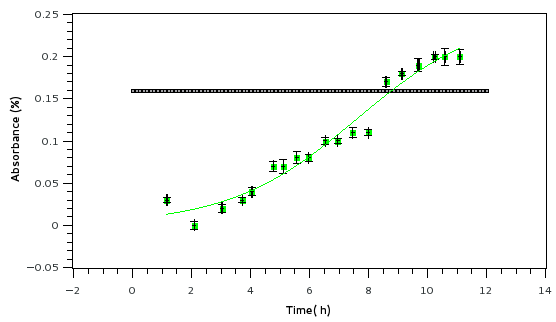
\includegraphics[width=\linewidth]{curvas/gra144.png}
  \caption{Curva de crecimiento para las cepas 144, 145 y 147}
  \label{fig:cur2}
   Para la 145  (día 1) se encontró un coeficiente de determinación de $r^2=0.994$.
   Los valores $a$, $b$ y $P_{0}$ de la sigmoidal ajustados se discutirán en la en informe final.
\end{figure}
\begin{figure}[h]
 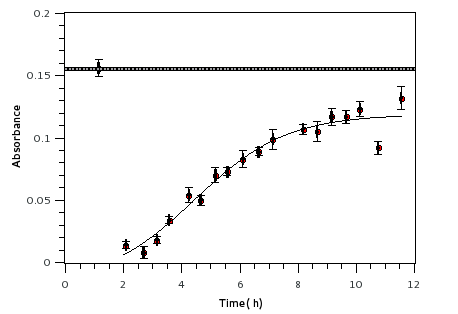
\includegraphics[width=\linewidth]{curvas/gra145dia1.png}
  \caption{Curvas de crecimiento para las cepas 144, 145 y 147}
  \label{fig:cur3}
\end{figure}
 Para la 145  (día 2) se encontró un coeficiente de determinación de $r^2=0.955$. 
 Los valores $a$, $b$ y $P_{0}$ de la sigmoidal ajustados se discutirán en la en informe final.
\begin{figure}[h]
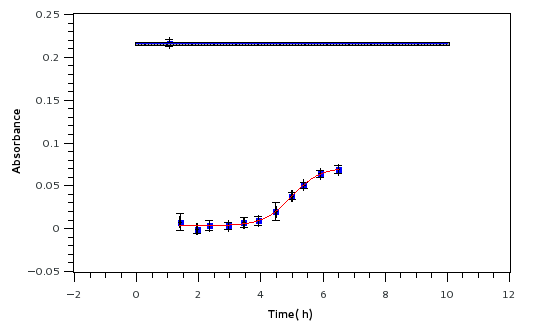
\includegraphics[width=\linewidth]{curvas/gra145dia2.png}
  \caption{Curvas de crecimiento para las cepas 144, 145 y 147}
  \label{fig:cur4}
\end{figure}
Debido a que la cepa 147 no creció en antibiótico se realiza otro experimento en el cual crece \textit{S. aureus} cepas 144 y 147 diluidas en LB a diferentes concentraciones de antibiótico, esto con el fin de determinar la concentración adecudad de antibótico suministrado a la 147. Se preparan 5 frascos con células 144, 5 con 147 y a cada frasco se le agregan diferentes concentraciones de eritromicina 0.4$\mu$g/mL, 0.8$\mu$g/mL, 1$\mu$g/mL, 1.2$\mu$g/mL y 1.4$\mu$g/mL y se dejan en el agitador (shaker) entre 4 y 6 horas \footnote{Este experimento fue realizado por el equipo del laboratorio de biofísica}\\
Los resultados obtenidos para el experimento fueron los mostrados en la figura \ref{fig:144_eri}.
\begin{figure}[h]
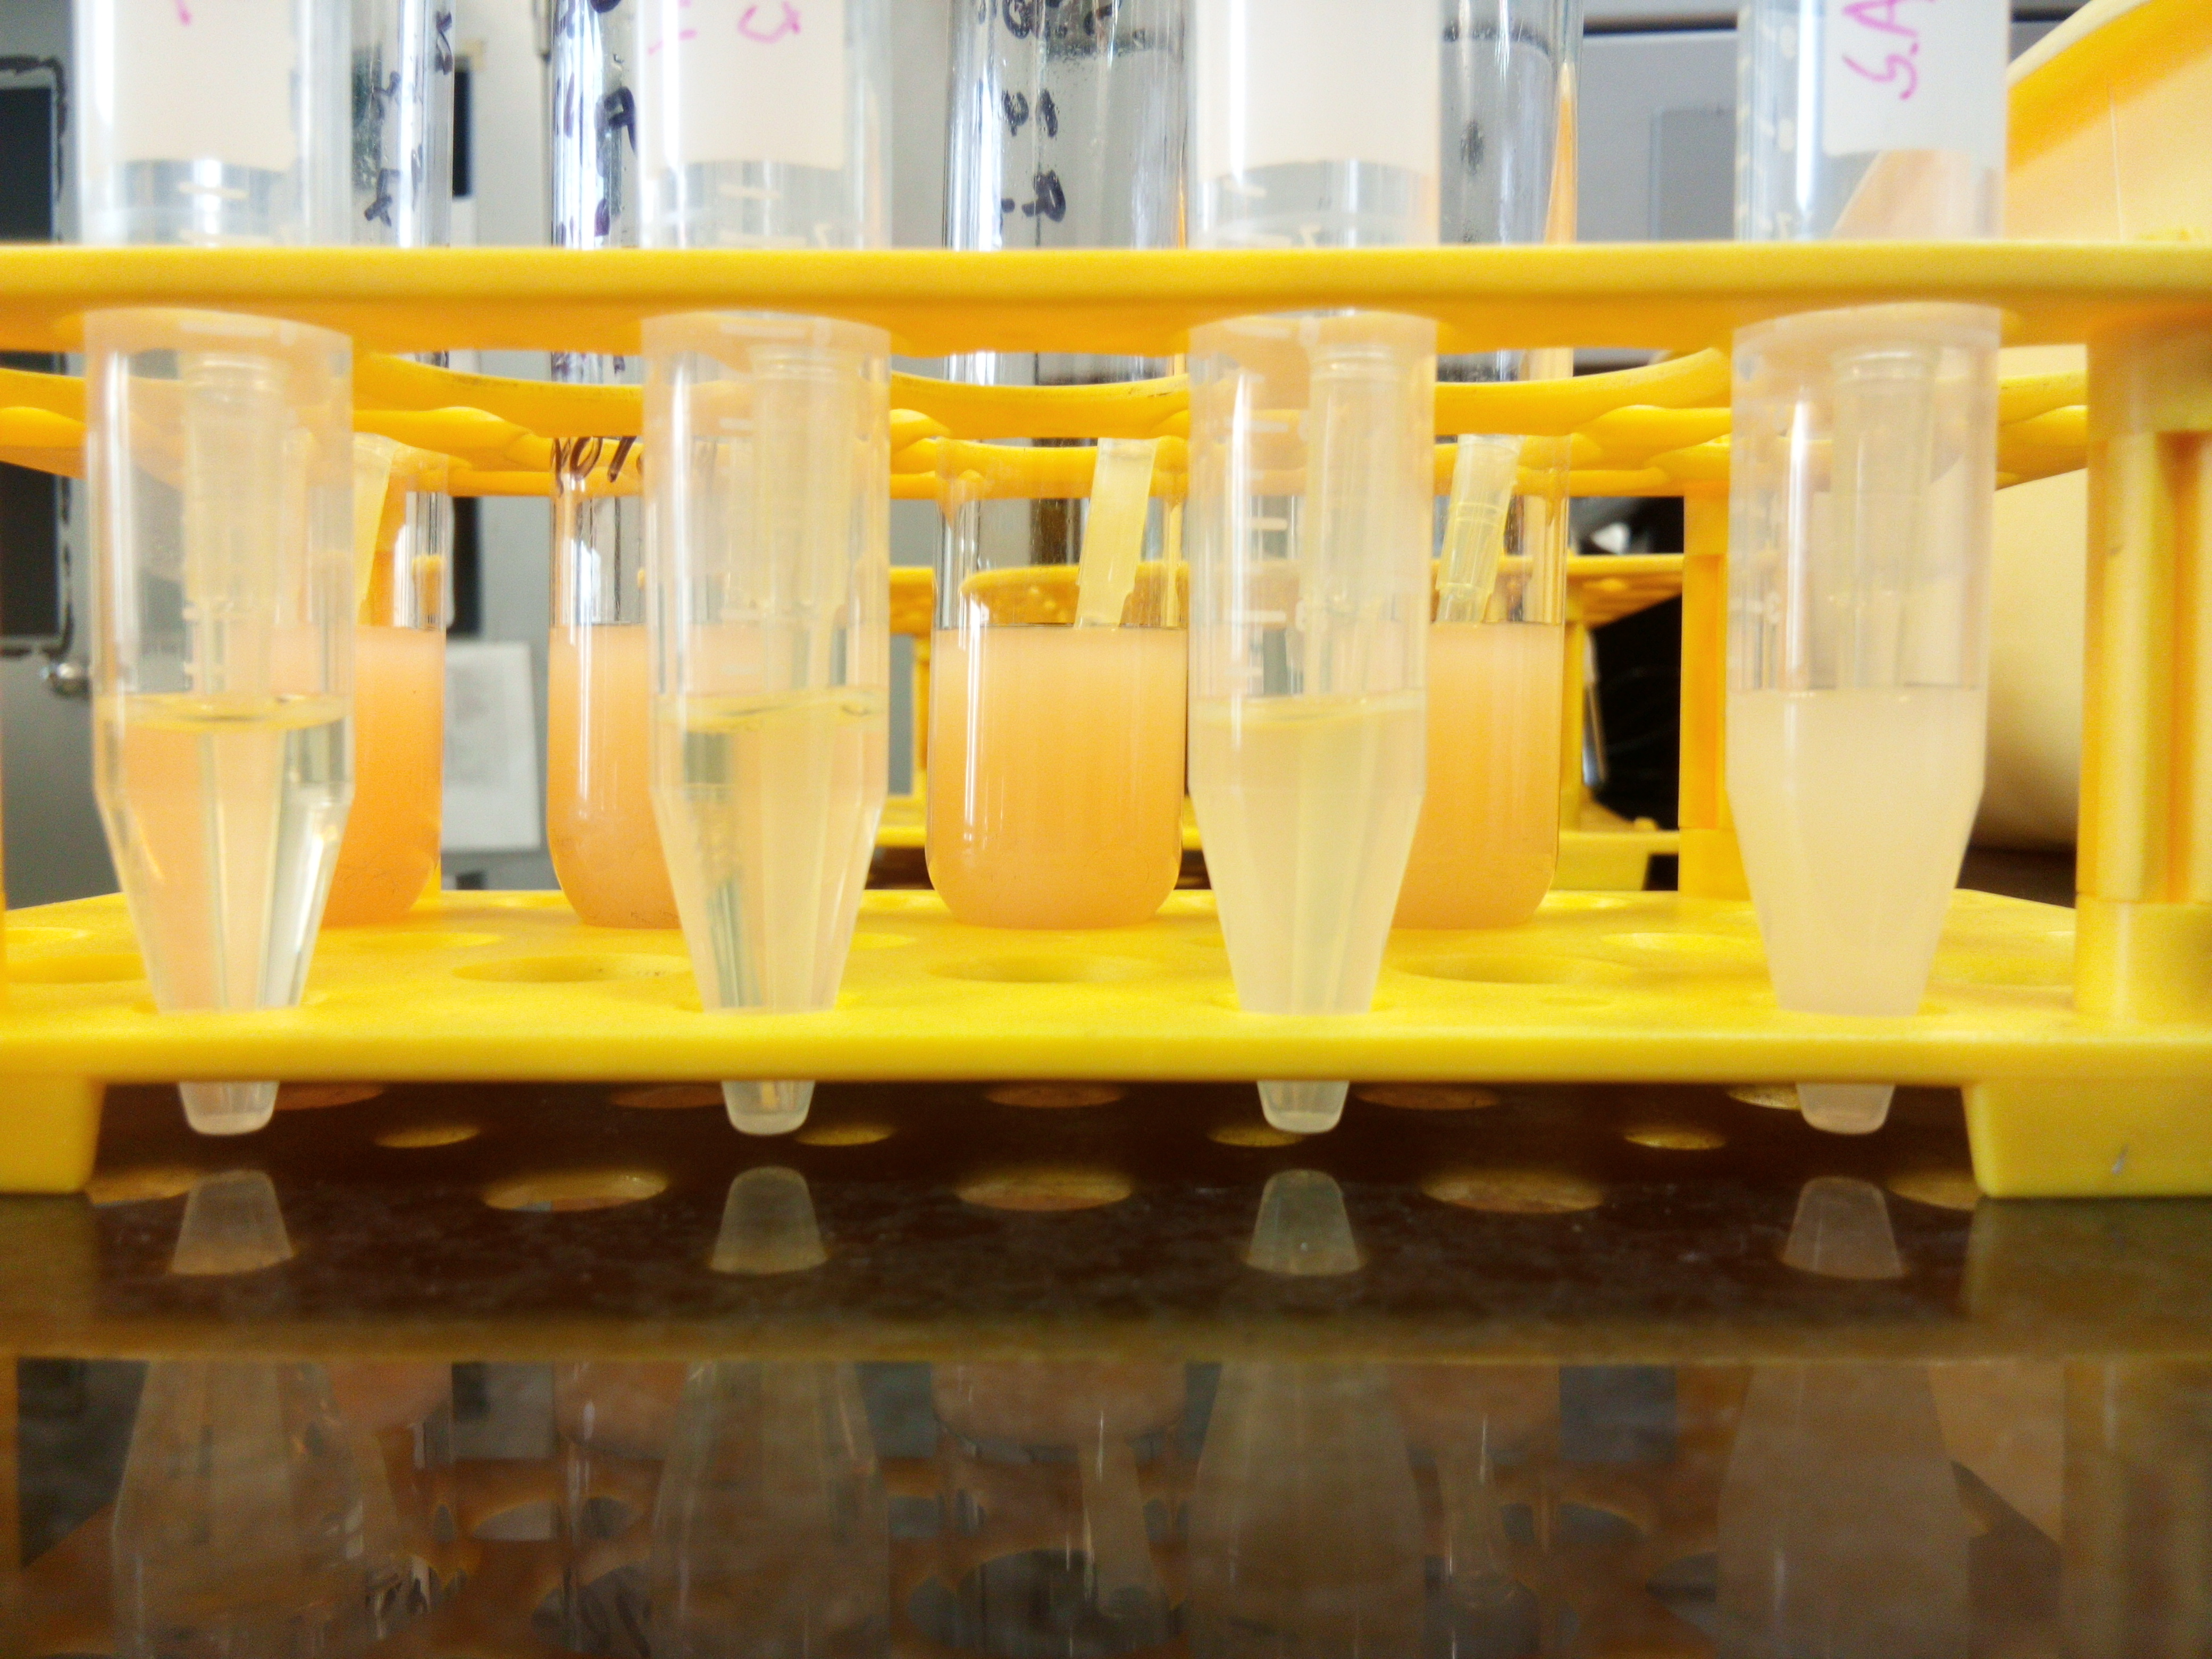
\includegraphics[scale=0.04]{144_eri.jpg}
  \caption{Crecimiento de la cepa 144 con diferentes concentraciones de  eritromicina. De derecha a izquierda 0.4$\mu$g/mL, 0.8$\mu$g/mL, 1$\mu$g/mL y 1.2$\mu$g/mL de  eritromicina.}
  \label{fig:144_eri}
\end{figure}
De la figura \ref{fig:144_eri} se puede concluir que la concentración de eritromicina más adecuada para crecer la cepa 147 es de 1$\mu$g/mL.
\subsection{Espectro en función de la Temperatura}
Para bicapas compuestas por DPPC se obtienen los espectros a 13\textdegree C, 17\textdegree C, 20\textdegree C, 25\textdegree C, 30\textdegree C y 35\textdegree C mostrados en el anexo. En la figura \ref{fig:espa13} se muestran los dos valles de interés para $T=13$\textdegree C.
\begin{figure}[h]
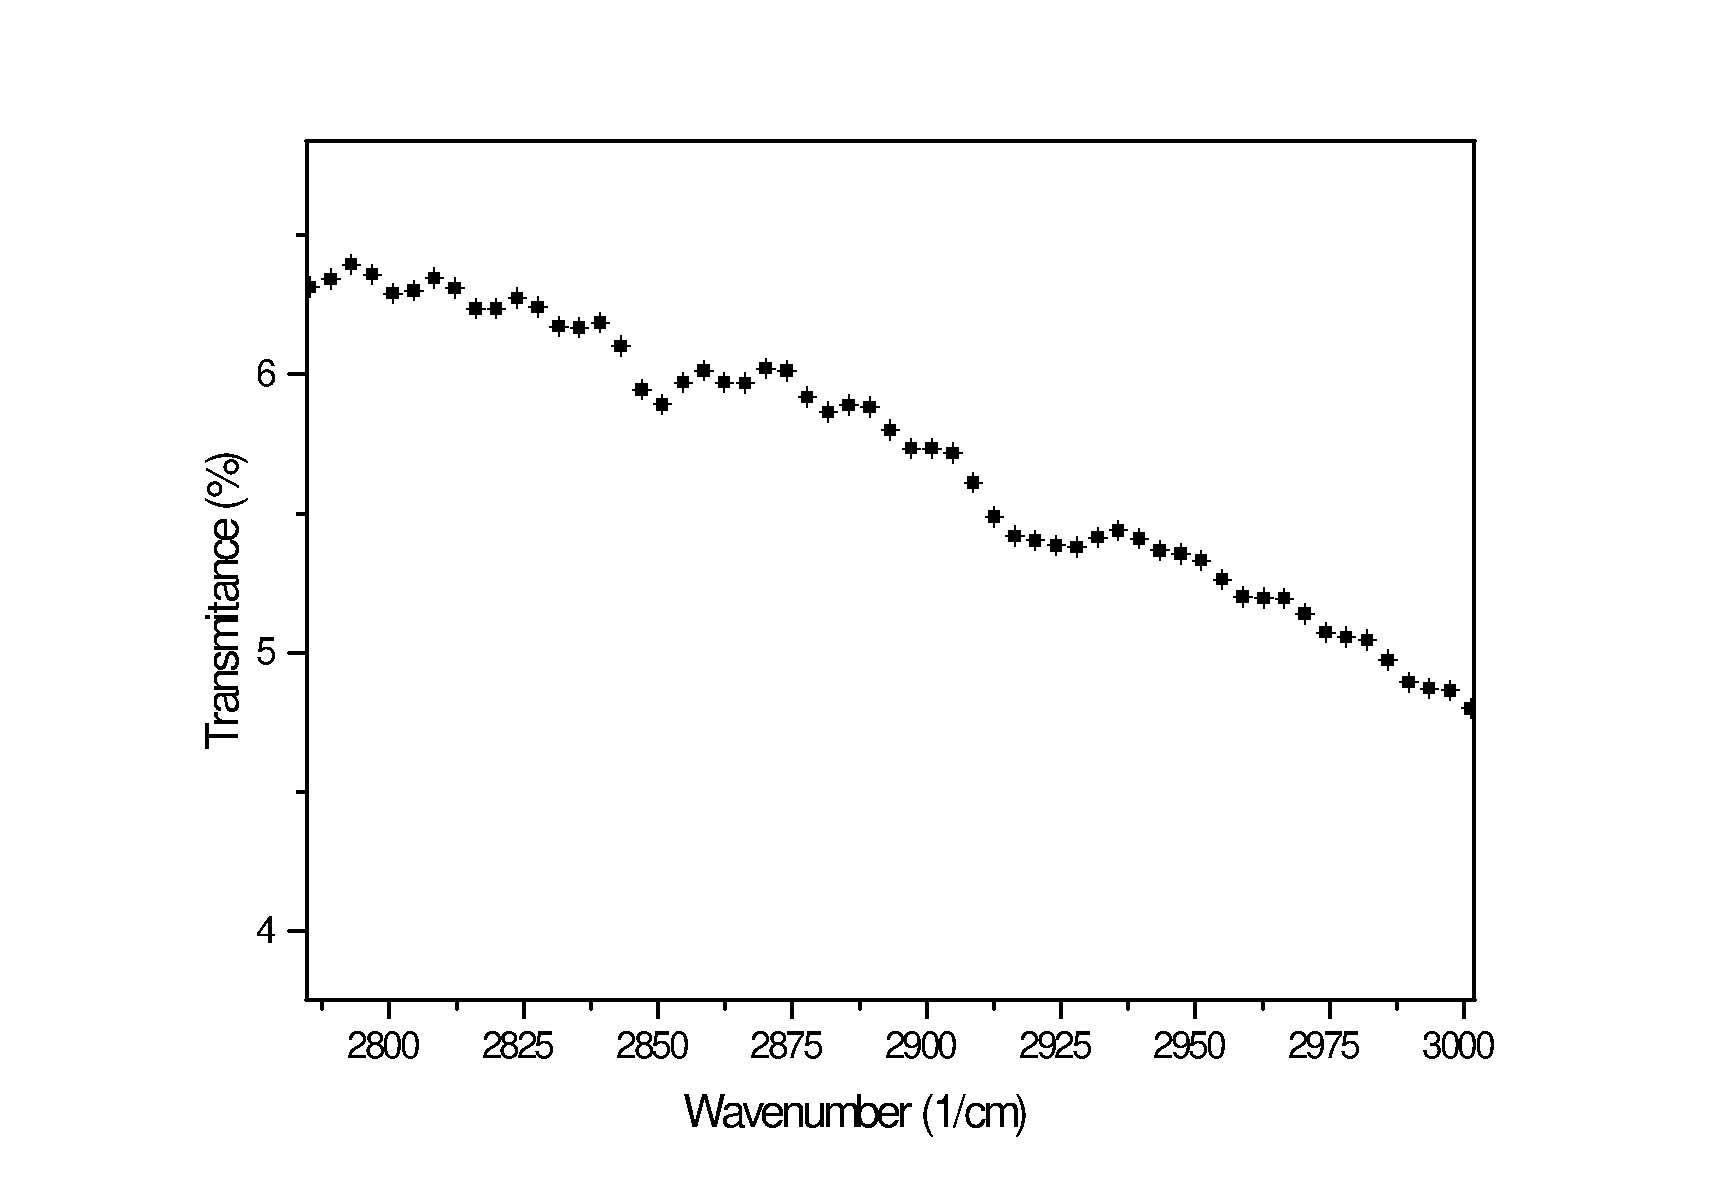
\includegraphics[scale=0.3]{FTIR/13C.pdf}
  \caption{Región del espectro de absorción para DPPC entre 2780 cm $^{-1}$ y 3000 cm $^{-1}$ a $T=13$\textdegree C.}
  \label{fig:espa13}
\end{figure}
Con el fin de conocer los valores experimentales de estos valles (que en adelante los llamaremos picos si consideramos el inverso del espectro de absorción) primero se calcula el inverso multiplicativo del espectro y luego se hallan mediante el método de la segunda derivada en $Qtiplot$. En la tabla 1 se muestran los valores y las posiciones de los picos encontrados para las 6 temperaturas:
\begin{table}[h]
    \centering
    \begin{tabular}{|c|c|}
         $(T\pm 1)$\textdegree C & $(k\pm 1\times 10^{-6}$cm$^-1$ \\\hline
        13 & 2850.790048\\
  17 & 2862.362944\\
  20&2862.362944\\
 25 &2877.793472\\
    \end{tabular}
    \caption{Número de onda del primer pico de la izquierda( Ver figuras 15 a 19 del anexo) para cada una de las temperaturas.}
    \label{tab:knumb}
\end{table}

De la tabla se observa que aunque hay un aumento en la temperatura de 20\textdegree C a 25\textdegree C también existe esta variación al pasar de 13\textdegree C a 17\textdegree C. Estas variaciones pueden deberse a  que el espectro presenta unas interferencias que pueden modificar los picos, estas son las ondulaciones mostradas en la gráfica \ref{fig:espa13}. Las interferencias son causadas por sitio dende se coloca la muestra en el control de temperatura.
%%%%%%%%%%%%%%%%%%%%%%%%%%%%%%%%%%%%%%%%%%%%%%%%%%%%%%%
\section{Conclusiones y Trabajo Futuro Documento}
De las gráficas para las curvas de crecimiento \ref{fig:cur1} se encuentra que a pesar de que los tiempos de crecimiento para la 145 no son los esperados, tanto para la 144 como para la 145 se observa un crecimiento con la forma de una curva sigmoidal.\\
Debido a que la cepa 147 no mostró crecimiento bajo las condiciones dadas en el marco experimental y a que la cepa 145 mostró diferencias para los dos días, se realizarán nuevamente las curvas de crecimiento para todas las cepas teniendo en cuenta que la concentración de eritromicina que se suministrará a las cepas 145 y 147 será de 1$\mu$g/mL.\\
En cuanto a los espectros aunque se observa un aumento en el número de onda contra la temperatura no se puede distinguir claramente la transición de fase de los liposomas hechos de DPPC. Se ha trabajado en disminuir la interferencia para encontrar encontrar el aumento abrupto en los picos alrededor de $23-24$ \textdegree C y se ya se ha disminuido la interferencia (resultados no mostrados aquí). Como ya se logró disminuir la intererencia se pasará a medir los espectros en función de la temperatura para las cepas 144, 145 y 147 de \textit{S. aureus} vivas.\\
\bibliographystyle{ieeetr}
\bibliography{references}
\vspace{1cm}
\pagebreak
\pagebreak
\section*{Anexo: Espectros obtenidos por FTIR para membranas de DPPC}
\begin{figure}[ht]
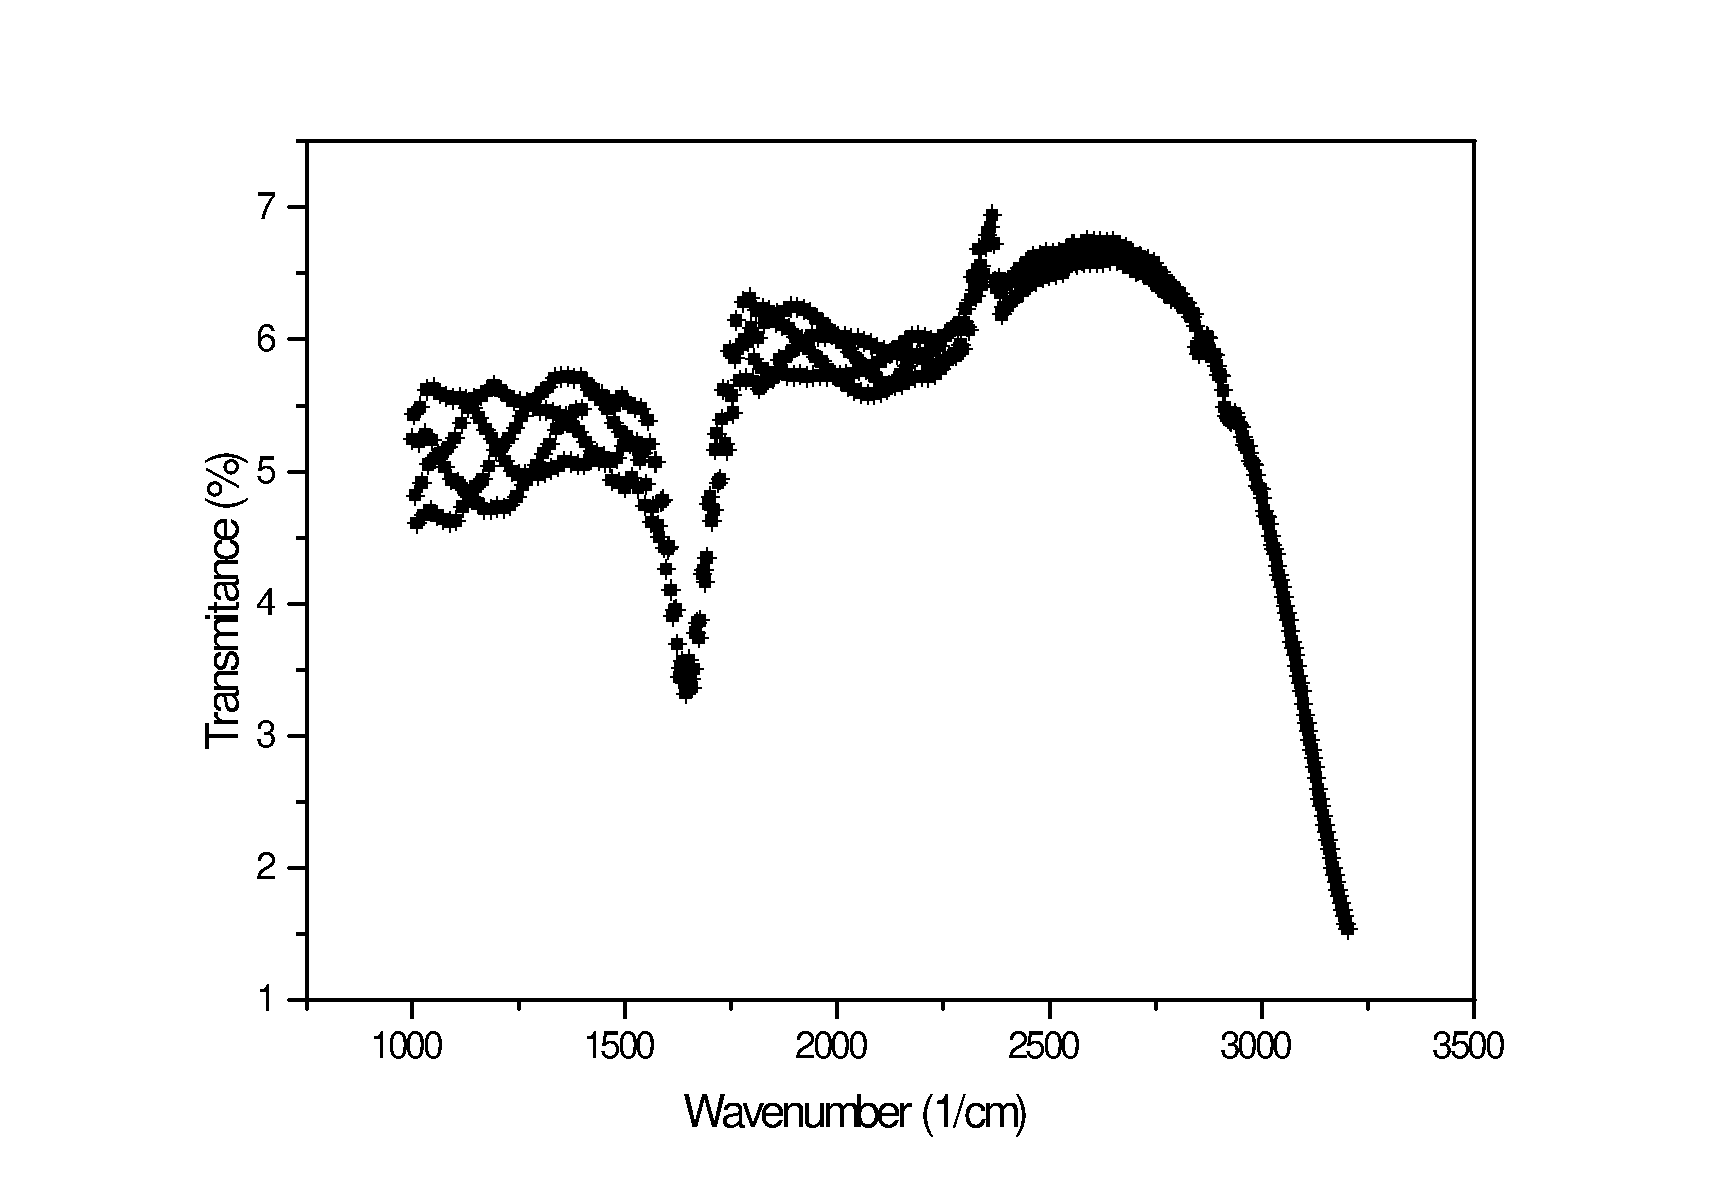
\includegraphics[scale=0.2]{FTIR/Graph1.pdf}
  \caption{Espectro de absorción para DPPC entre 1000 cm $^{-1}$ y 3300 cm $^{-1}$ a $T=13$\textdegree C.}
  \label{fig:13}
\end{figure}
\begin{figure}[ht]
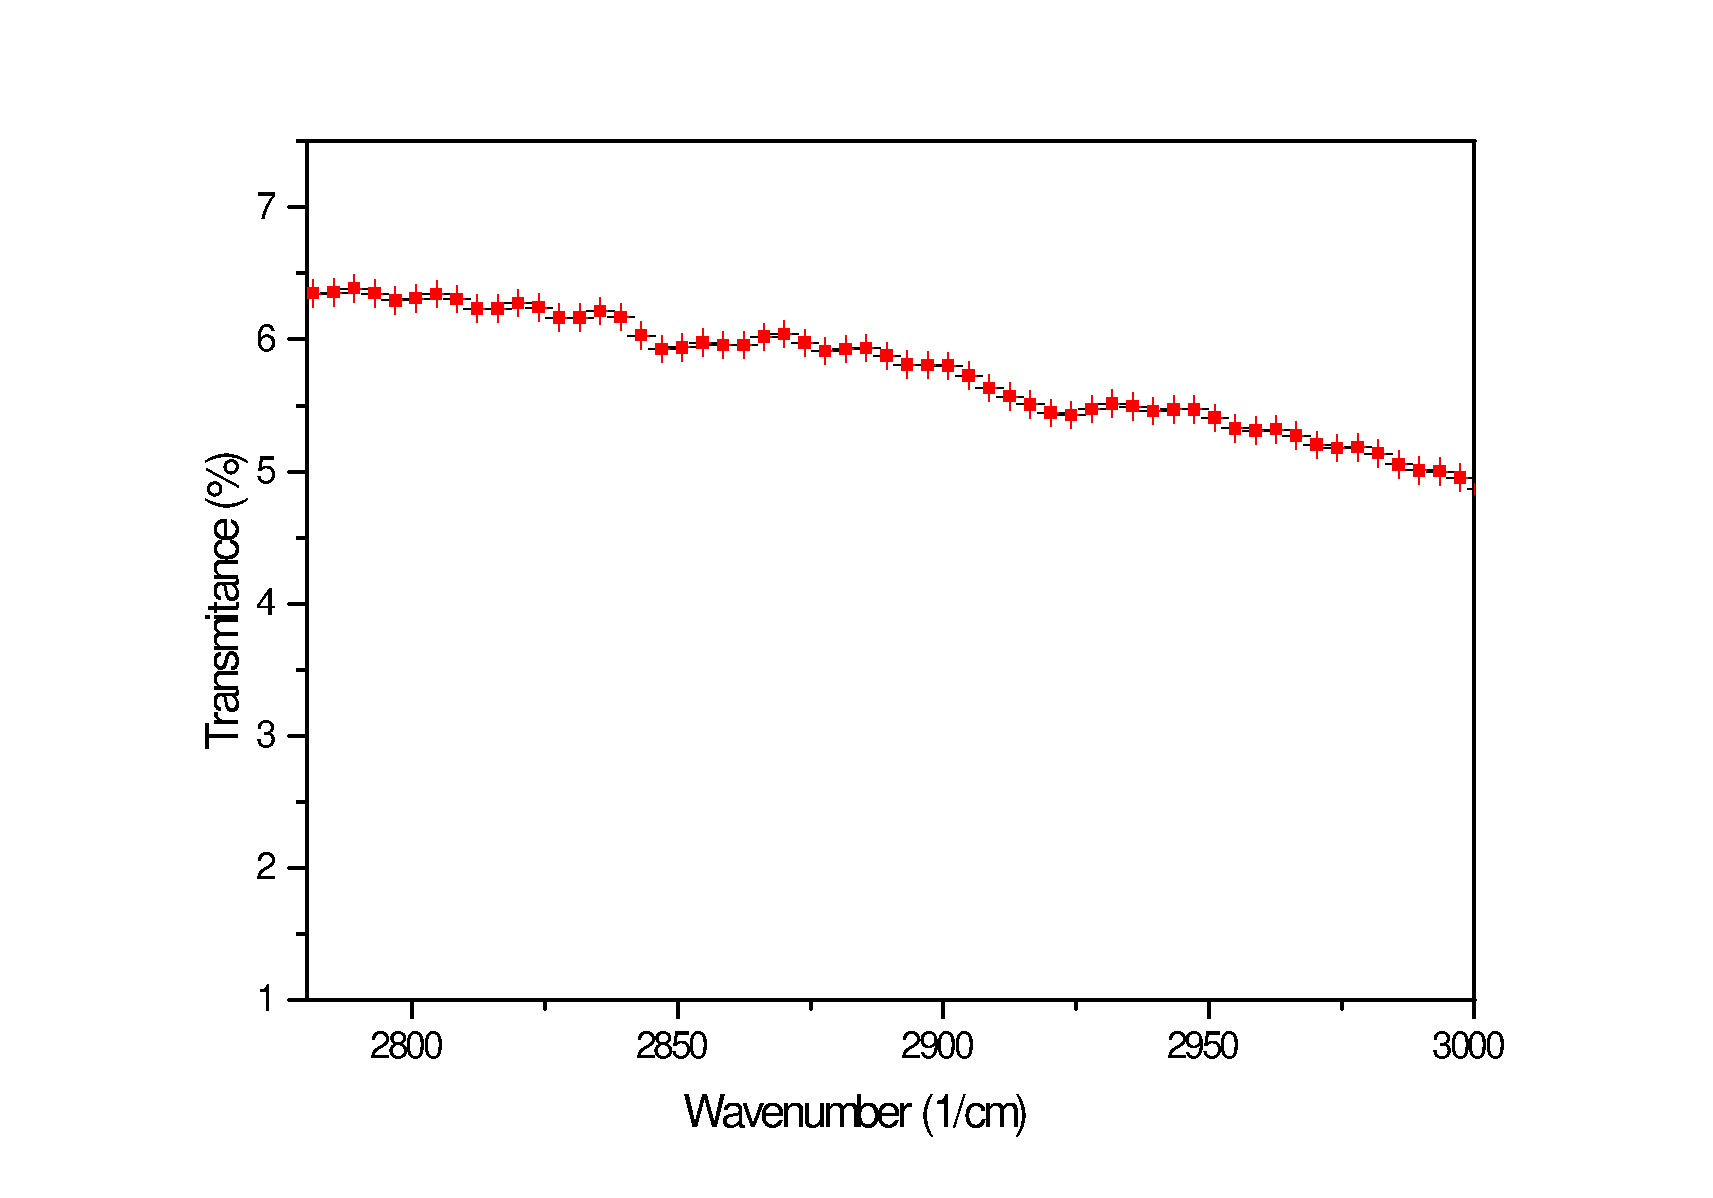
\includegraphics[scale=0.25]{FTIR/17C.pdf}
  \caption{Región del espectro de absorción para DPPC entre 2780 cm $^{-1}$ y 3000 cm $^{-1}$ a $T=17$\textdegree C.}
  \label{fig:espa17}
\end{figure}
\begin{figure}[ht]
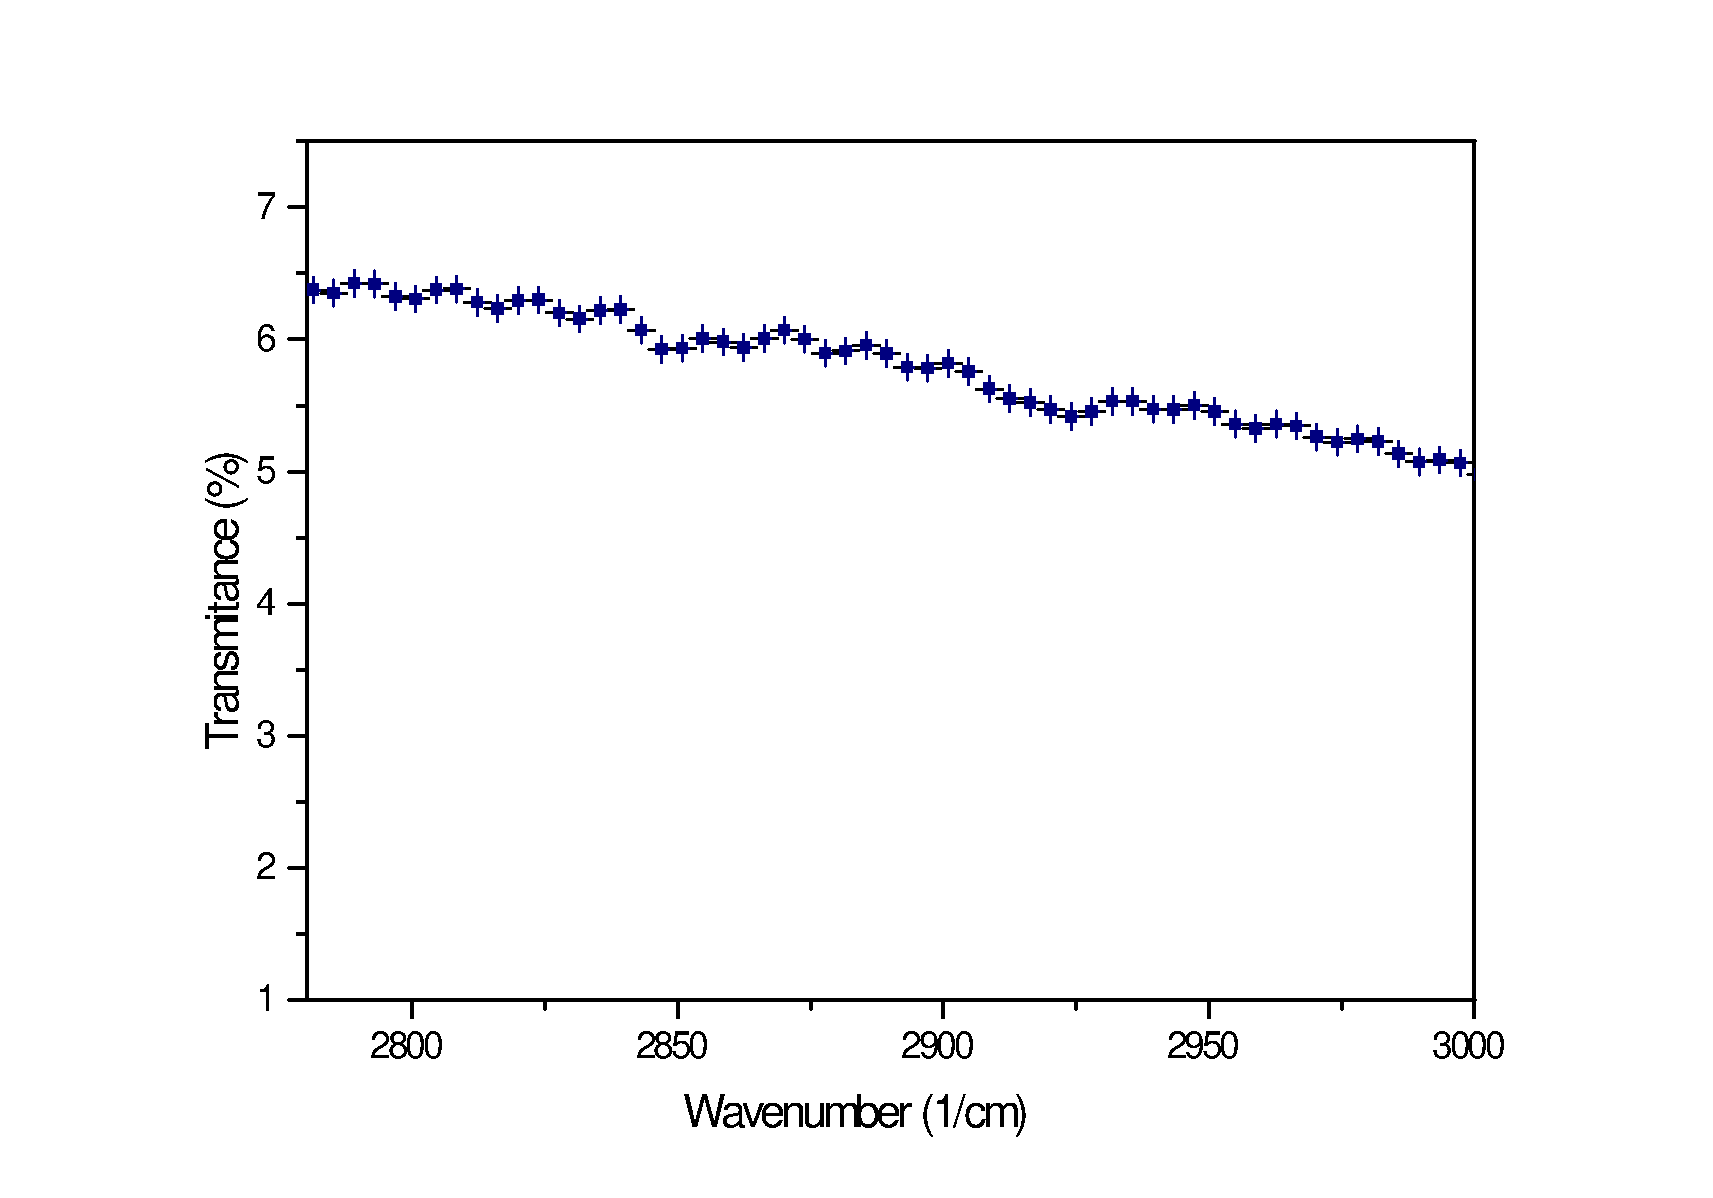
\includegraphics[scale=0.25]{FTIR/20C.pdf}
  \caption{Región del espectro de absorción para DPPC entre 2780 cm $^{-1}$ y 3000 cm $^{-1}$ a $T=20$\textdegree C.}
  \label{fig:espa20}
\end{figure}
\begin{figure}[ht]
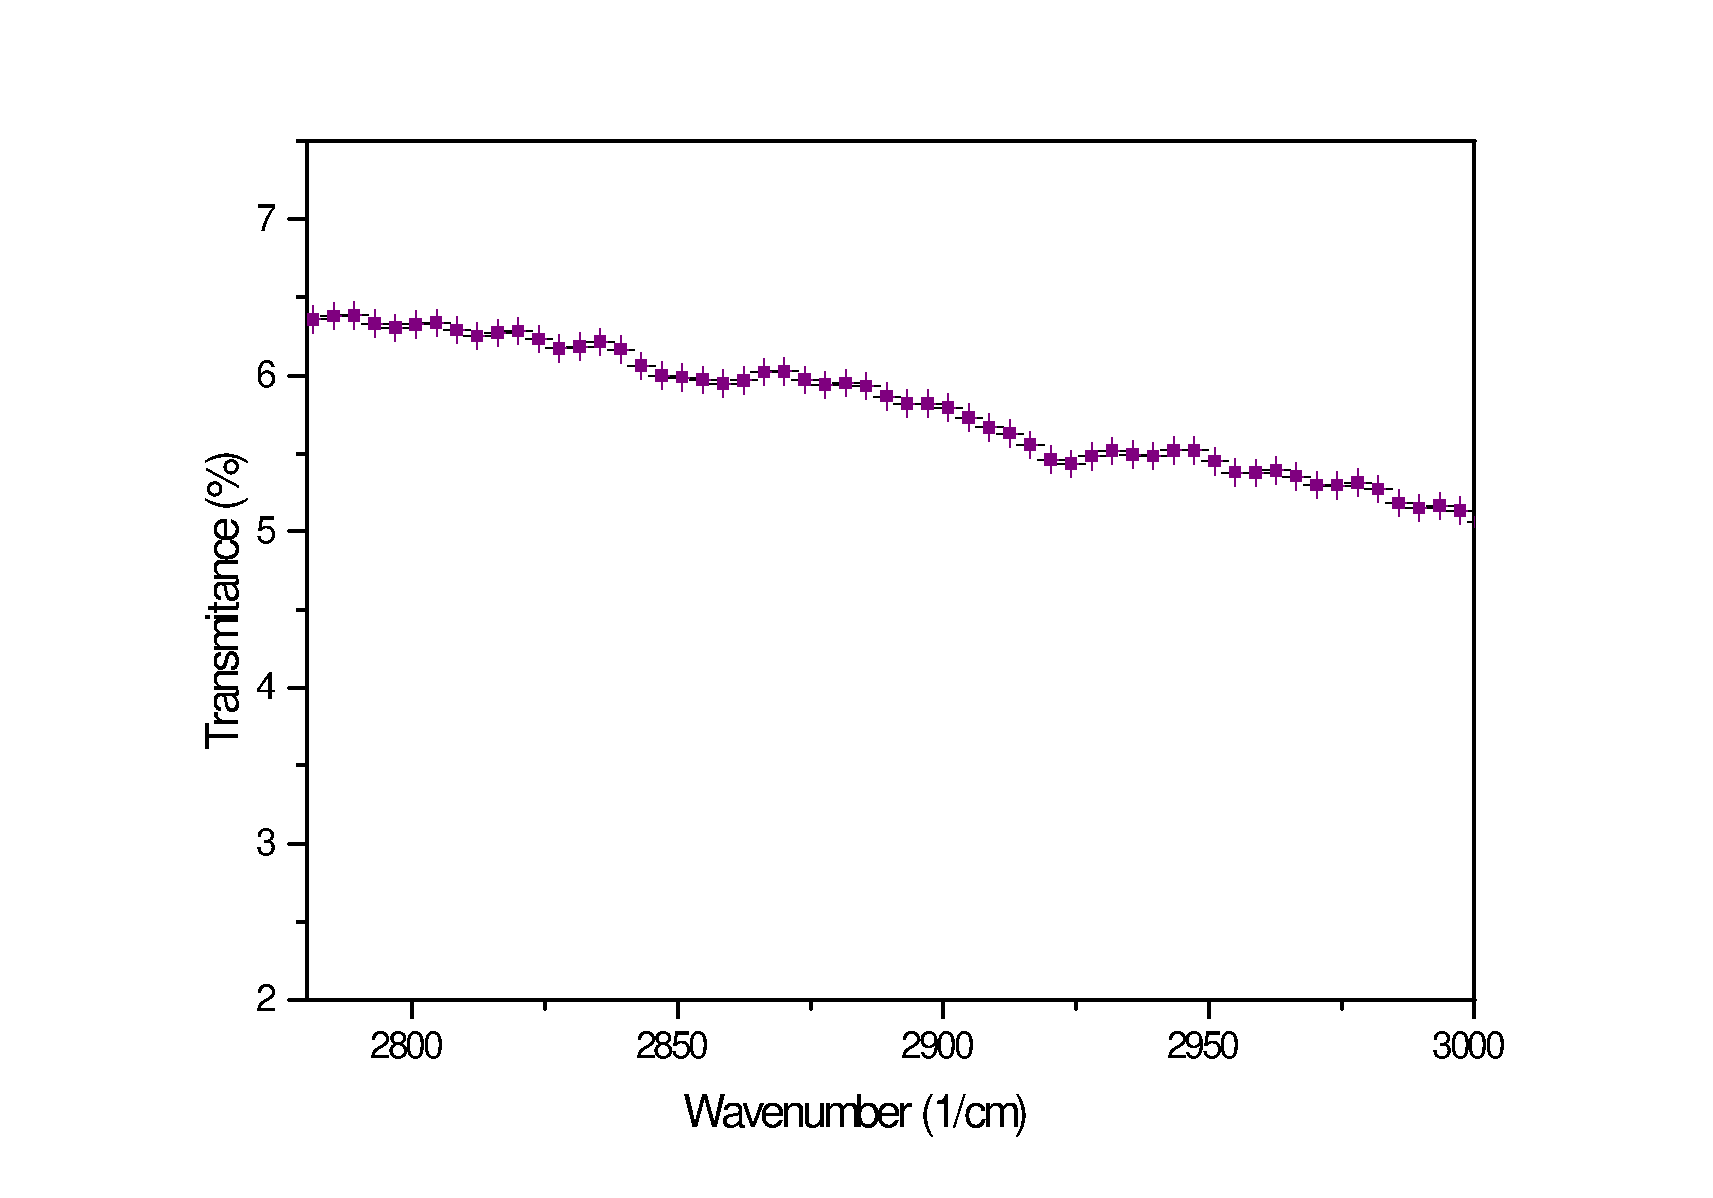
\includegraphics[scale=0.25]{FTIR/25C.pdf}
  \caption{Región del espectro de absorción para DPPC entre 2780 cm $^{-1}$ y 3000 cm $^{-1}$ a $T=25$\textdegree C.}
  \label{fig:espa25}
\end{figure}
\begin{figure}[ht]
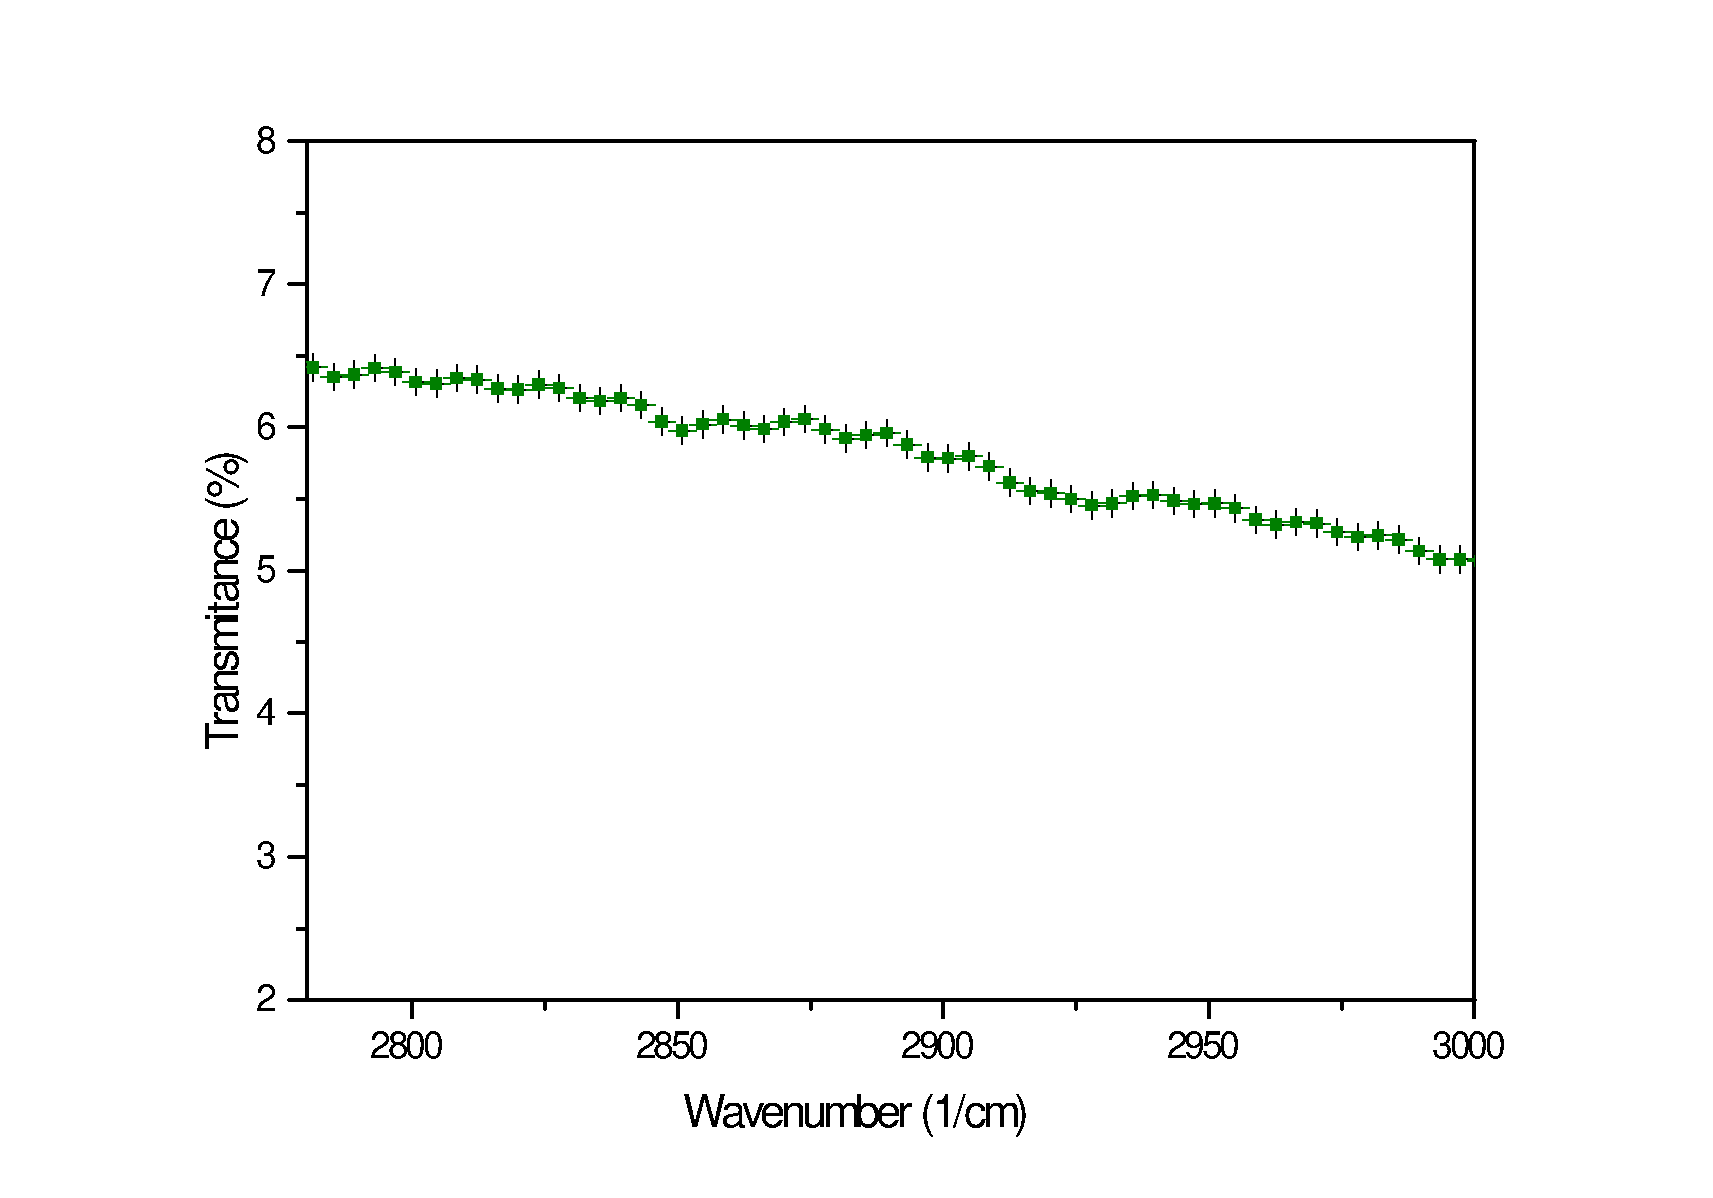
\includegraphics[scale=0.25]{FTIR/30C.pdf}
  \caption{Región del espectro de absorción para DPPC entre 2780 cm $^{-1}$ y 3000 cm $^{-1}$ a $T=30$\textdegree C.}
  \label{fig:espa30}
\end{figure}
\begin{figure}[ht]
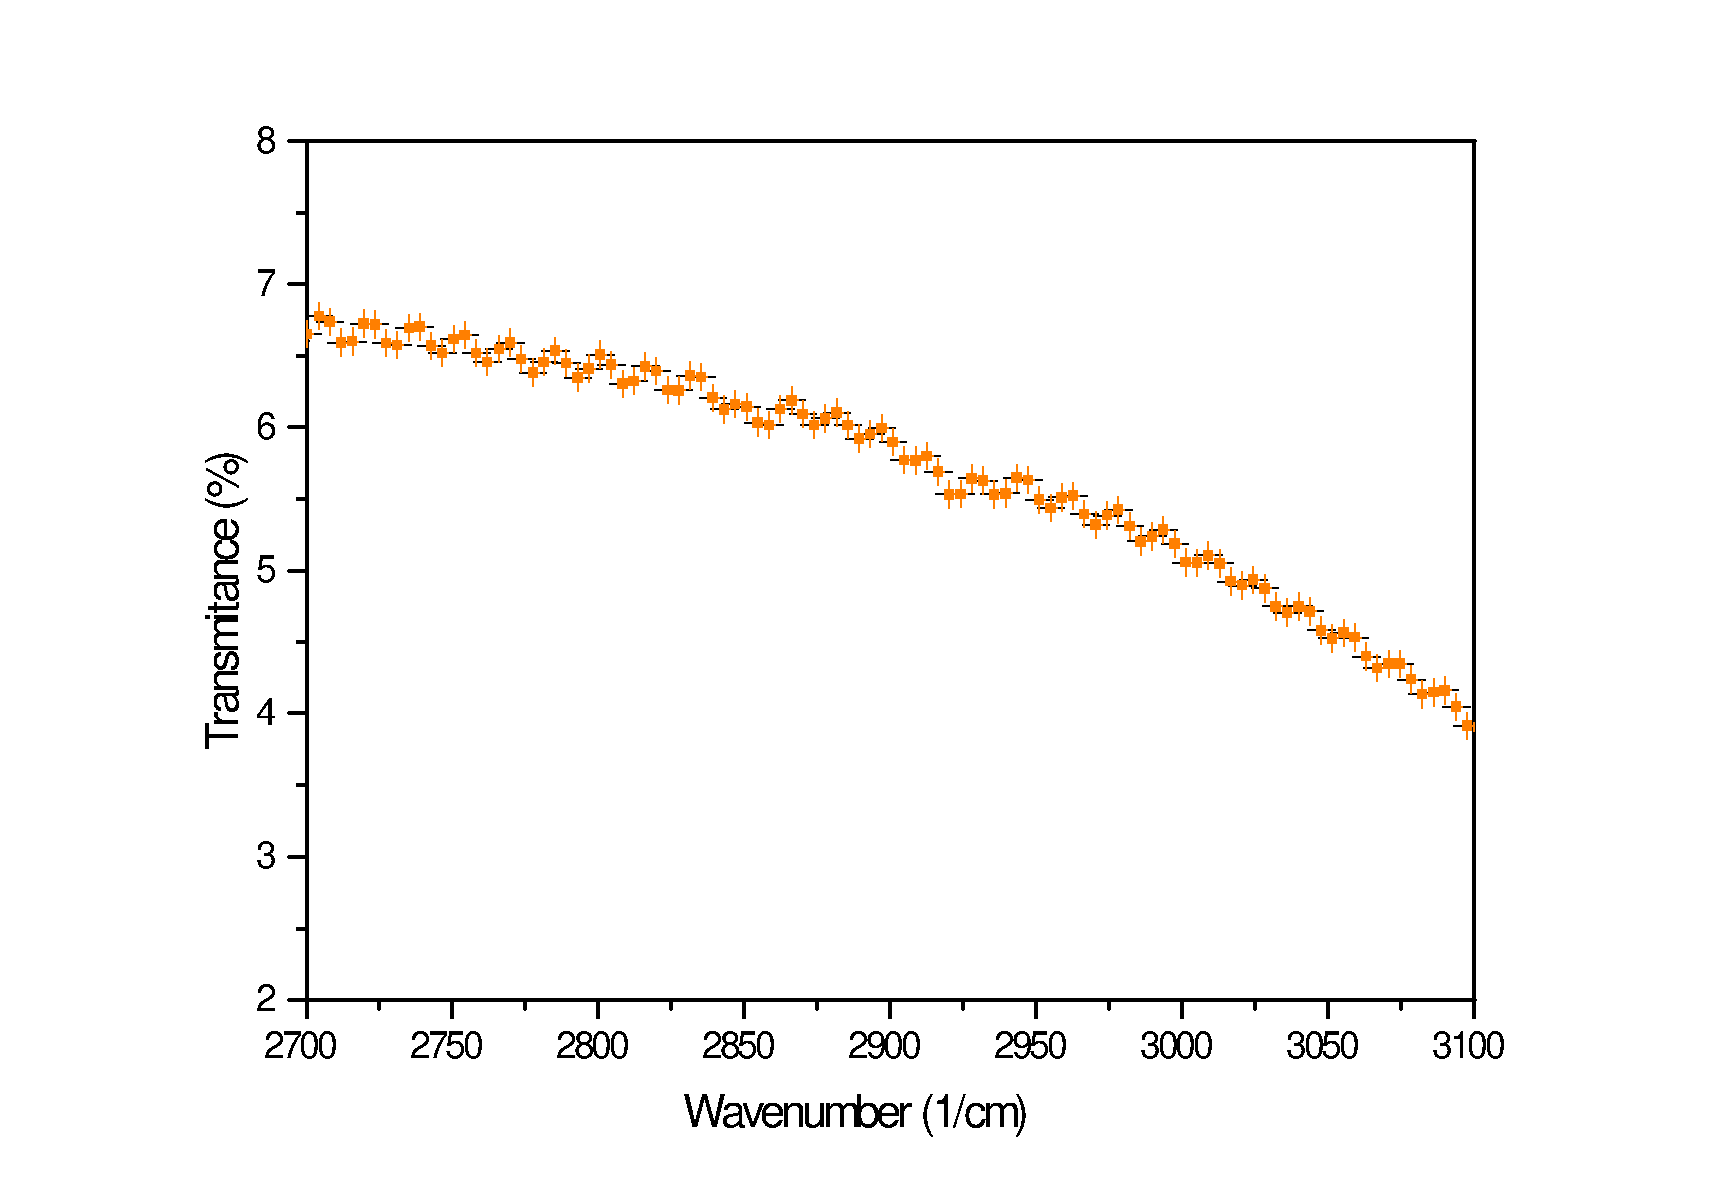
\includegraphics[scale=0.25]{FTIR/35C.pdf}
  \caption{Región del espectro de absorción para DPPC entre 2780 cm $^{-1}$ y 3000 cm $^{-1}$ a $T=35$\textdegree C.}
  \label{fig:espa35}
\end{figure}


\end{document}


% ****** End of file apssamp.tex ******
